\subsection{1. Thiết kế hệ thống}

\indent\indent Quy trình tổng quát của hệ thống \textit{SybilSignal} được thiết kế nhằm giải quyết bài toán phát hiện tài khoản giả mạo thông qua hai phân hệ chính hoạt động bổ trợ lẫn nhau: \textit{Phân hệ học biểu diễn và gán nhãn} chịu trách nhiệm kiến tạo dữ liệu và gán nhãn tự động; và \textit{Phân hệ đánh giá rủi ro} thực hiện nhiệm vụ dự đoán và diễn giải kết quả theo thời gian thực.\vspace{0.3cm}

Kiến trúc tổng thể và luồng xử lý dữ liệu khép kín giữa các module được minh họa trực quan tại \textbf{Hình \ref{fig:SystemOverview}}.

\begin{figure}[H]
    \centering
    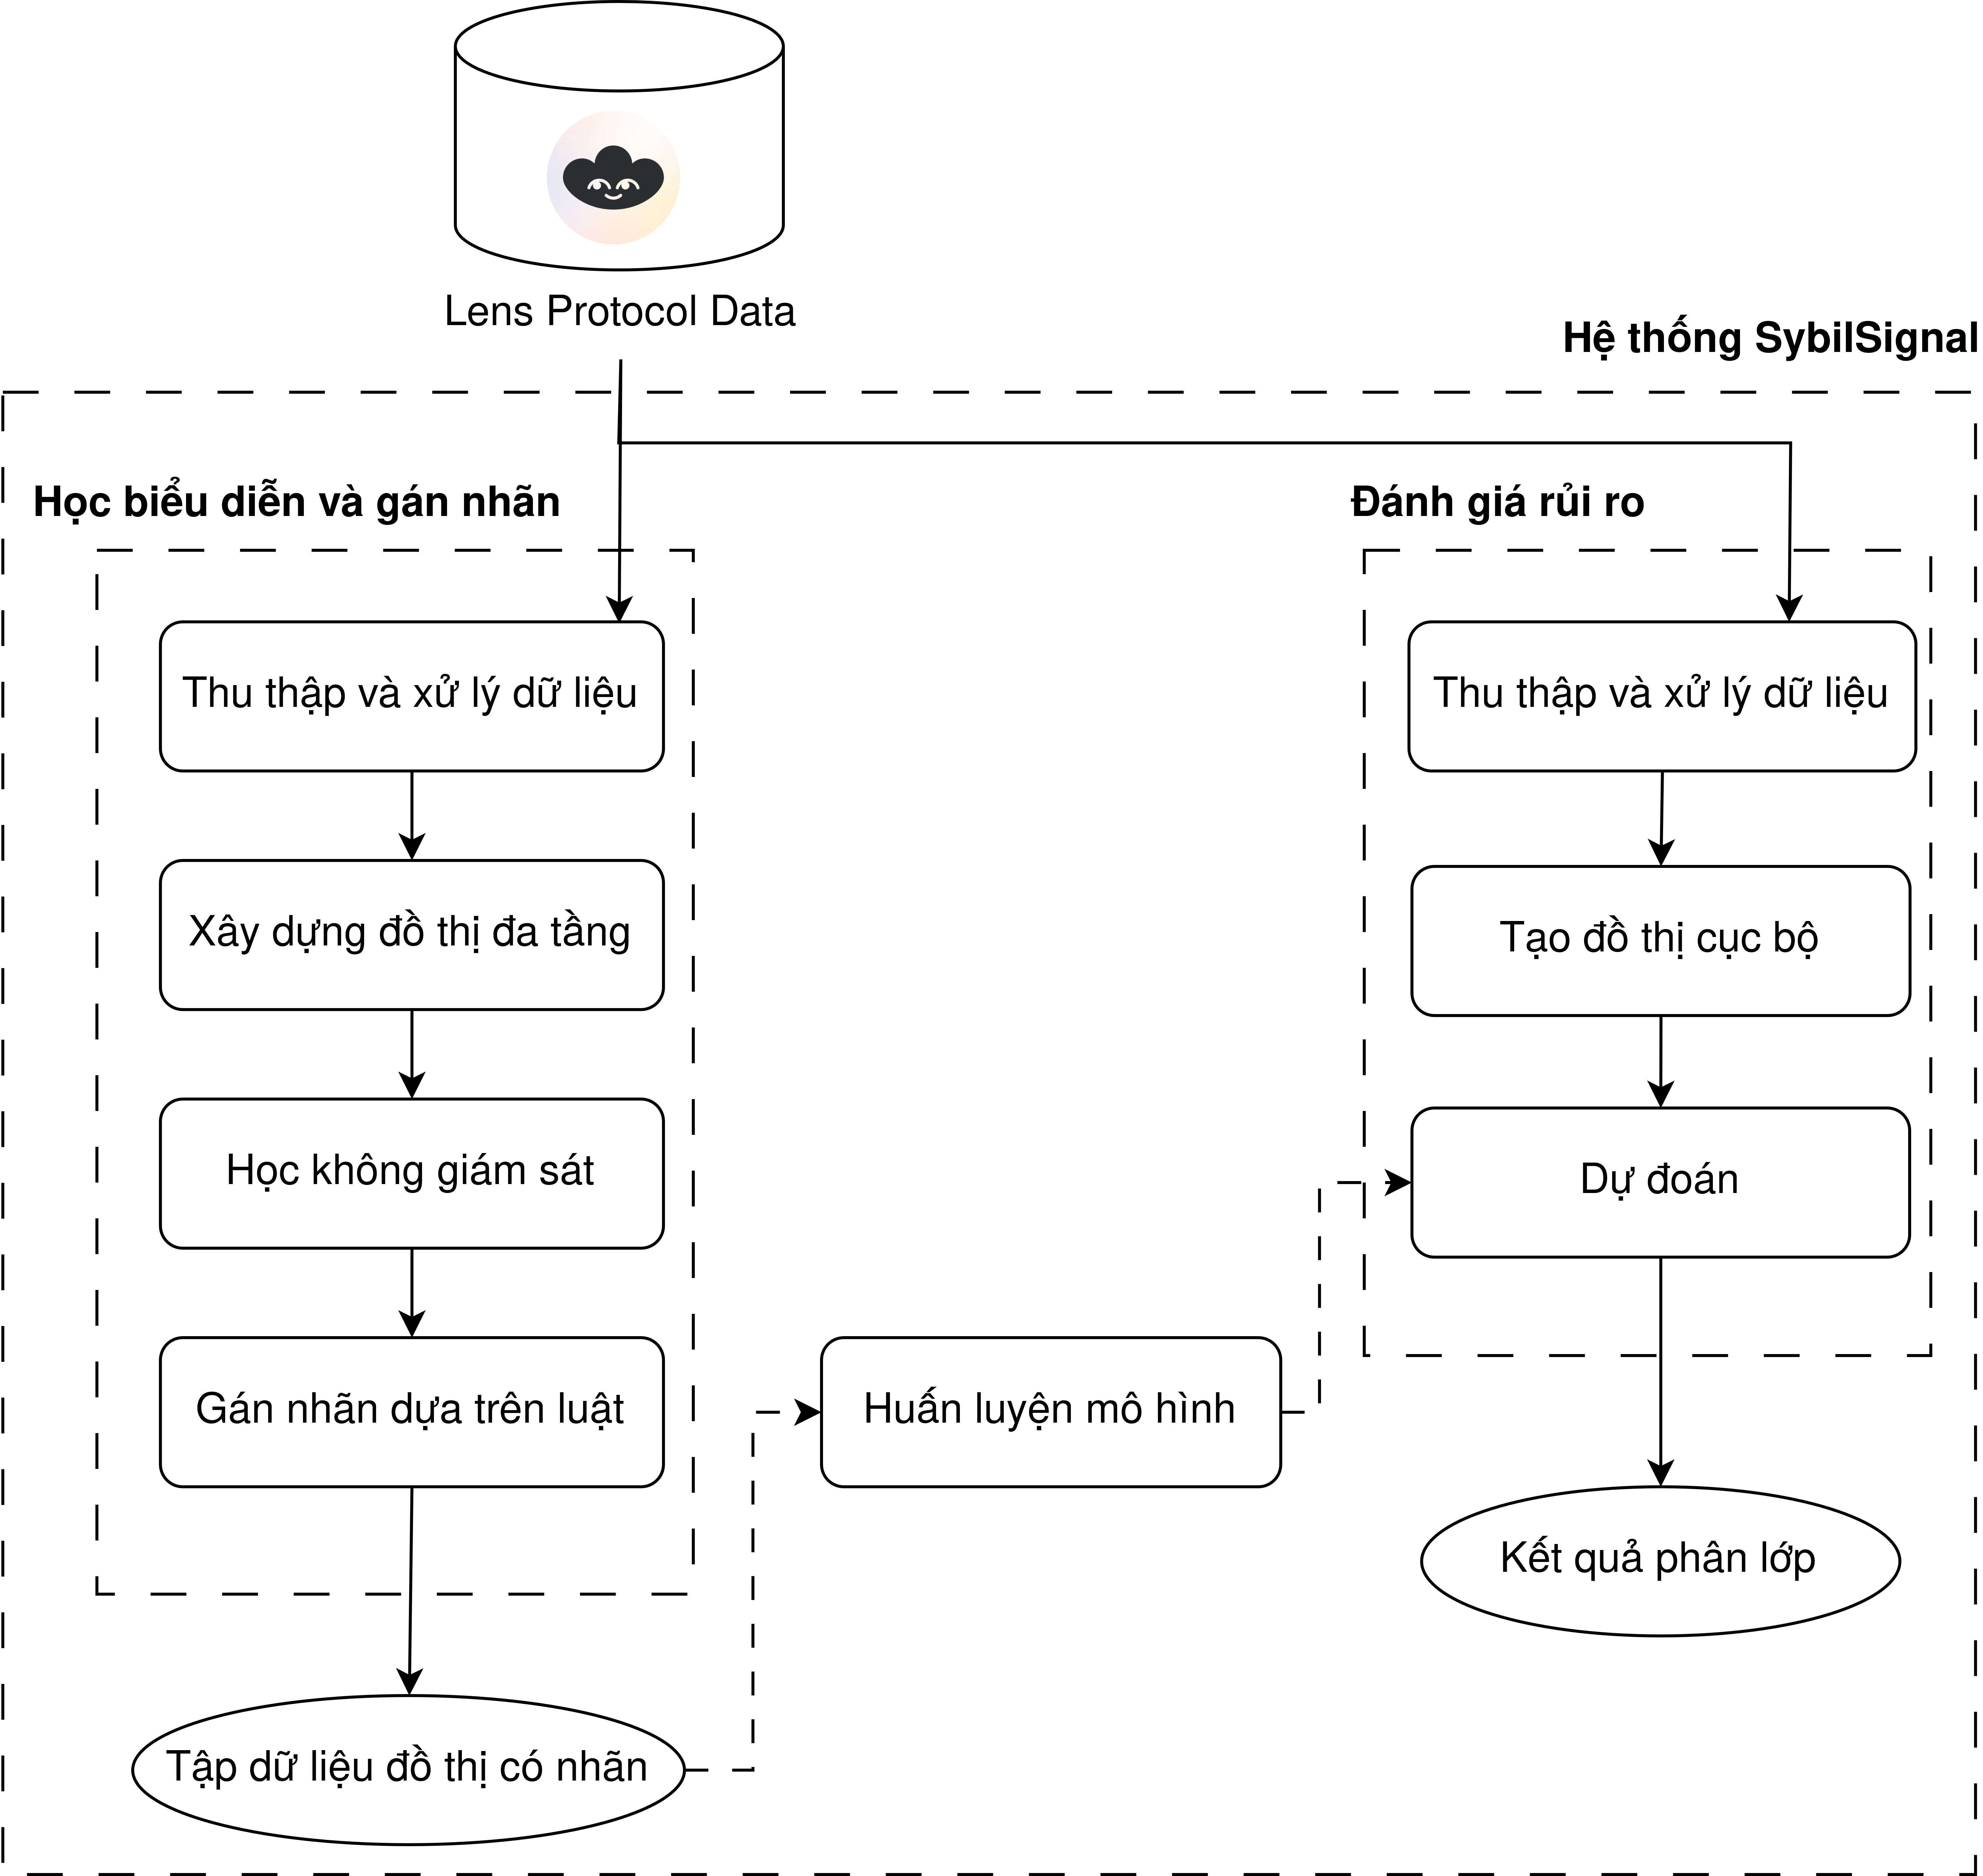
\includegraphics[width=0.85\linewidth]{images/part-02/chap-02/sec-01/SystemOverview.png} 
    \vspace{0.2cm}
    \caption{Sơ đồ kiến trúc tổng thể của hệ thống SybilSignal}
    \label{fig:SystemOverview}
\end{figure}

Dựa trên sơ đồ kiến trúc này, nội dung các phần tiếp theo sẽ đi sâu vào đặc tả chi tiết quy trình thiết kế, cơ sở toán học và cấu hình kỹ thuật của từng phân hệ thành phần.

\subsubsection{1.1. Quy trình thu thập và xây dựng dữ liệu đồ thị đa tầng nhận thức ràng buộc}

\indent\indent Trước khi đưa vào huấn luyện các mô hình học sâu đồ thị, dữ liệu thô từ mạng xã hội phi tập trung cần trải qua một quy trình tiền xử lý phức tạp. Mục tiêu của giai đoạn này là chuyển đổi các bản ghi cơ sở dữ liệu phẳng thành một cấu trúc đồ thị đa quan hệ có hướng, trong đó mỗi nút và cạnh đều mang lượng thông tin ngữ nghĩa và toán học cao nhất.\vspace{0.3cm}

\indent Sơ đồ luồng xử lý thu thập và kiến tạo đồ thị được minh họa tại \textbf{Hình \ref{fig:GraphBuilder}}, bao gồm hai nhánh xử lý song song và cơ chế hoạt động như sau:
\begin{figure}[H]
    \centering
    % Hãy đổi tên file ảnh dưới đây cho khớp với tên file ảnh của bạn trong thư mục Overleaf
    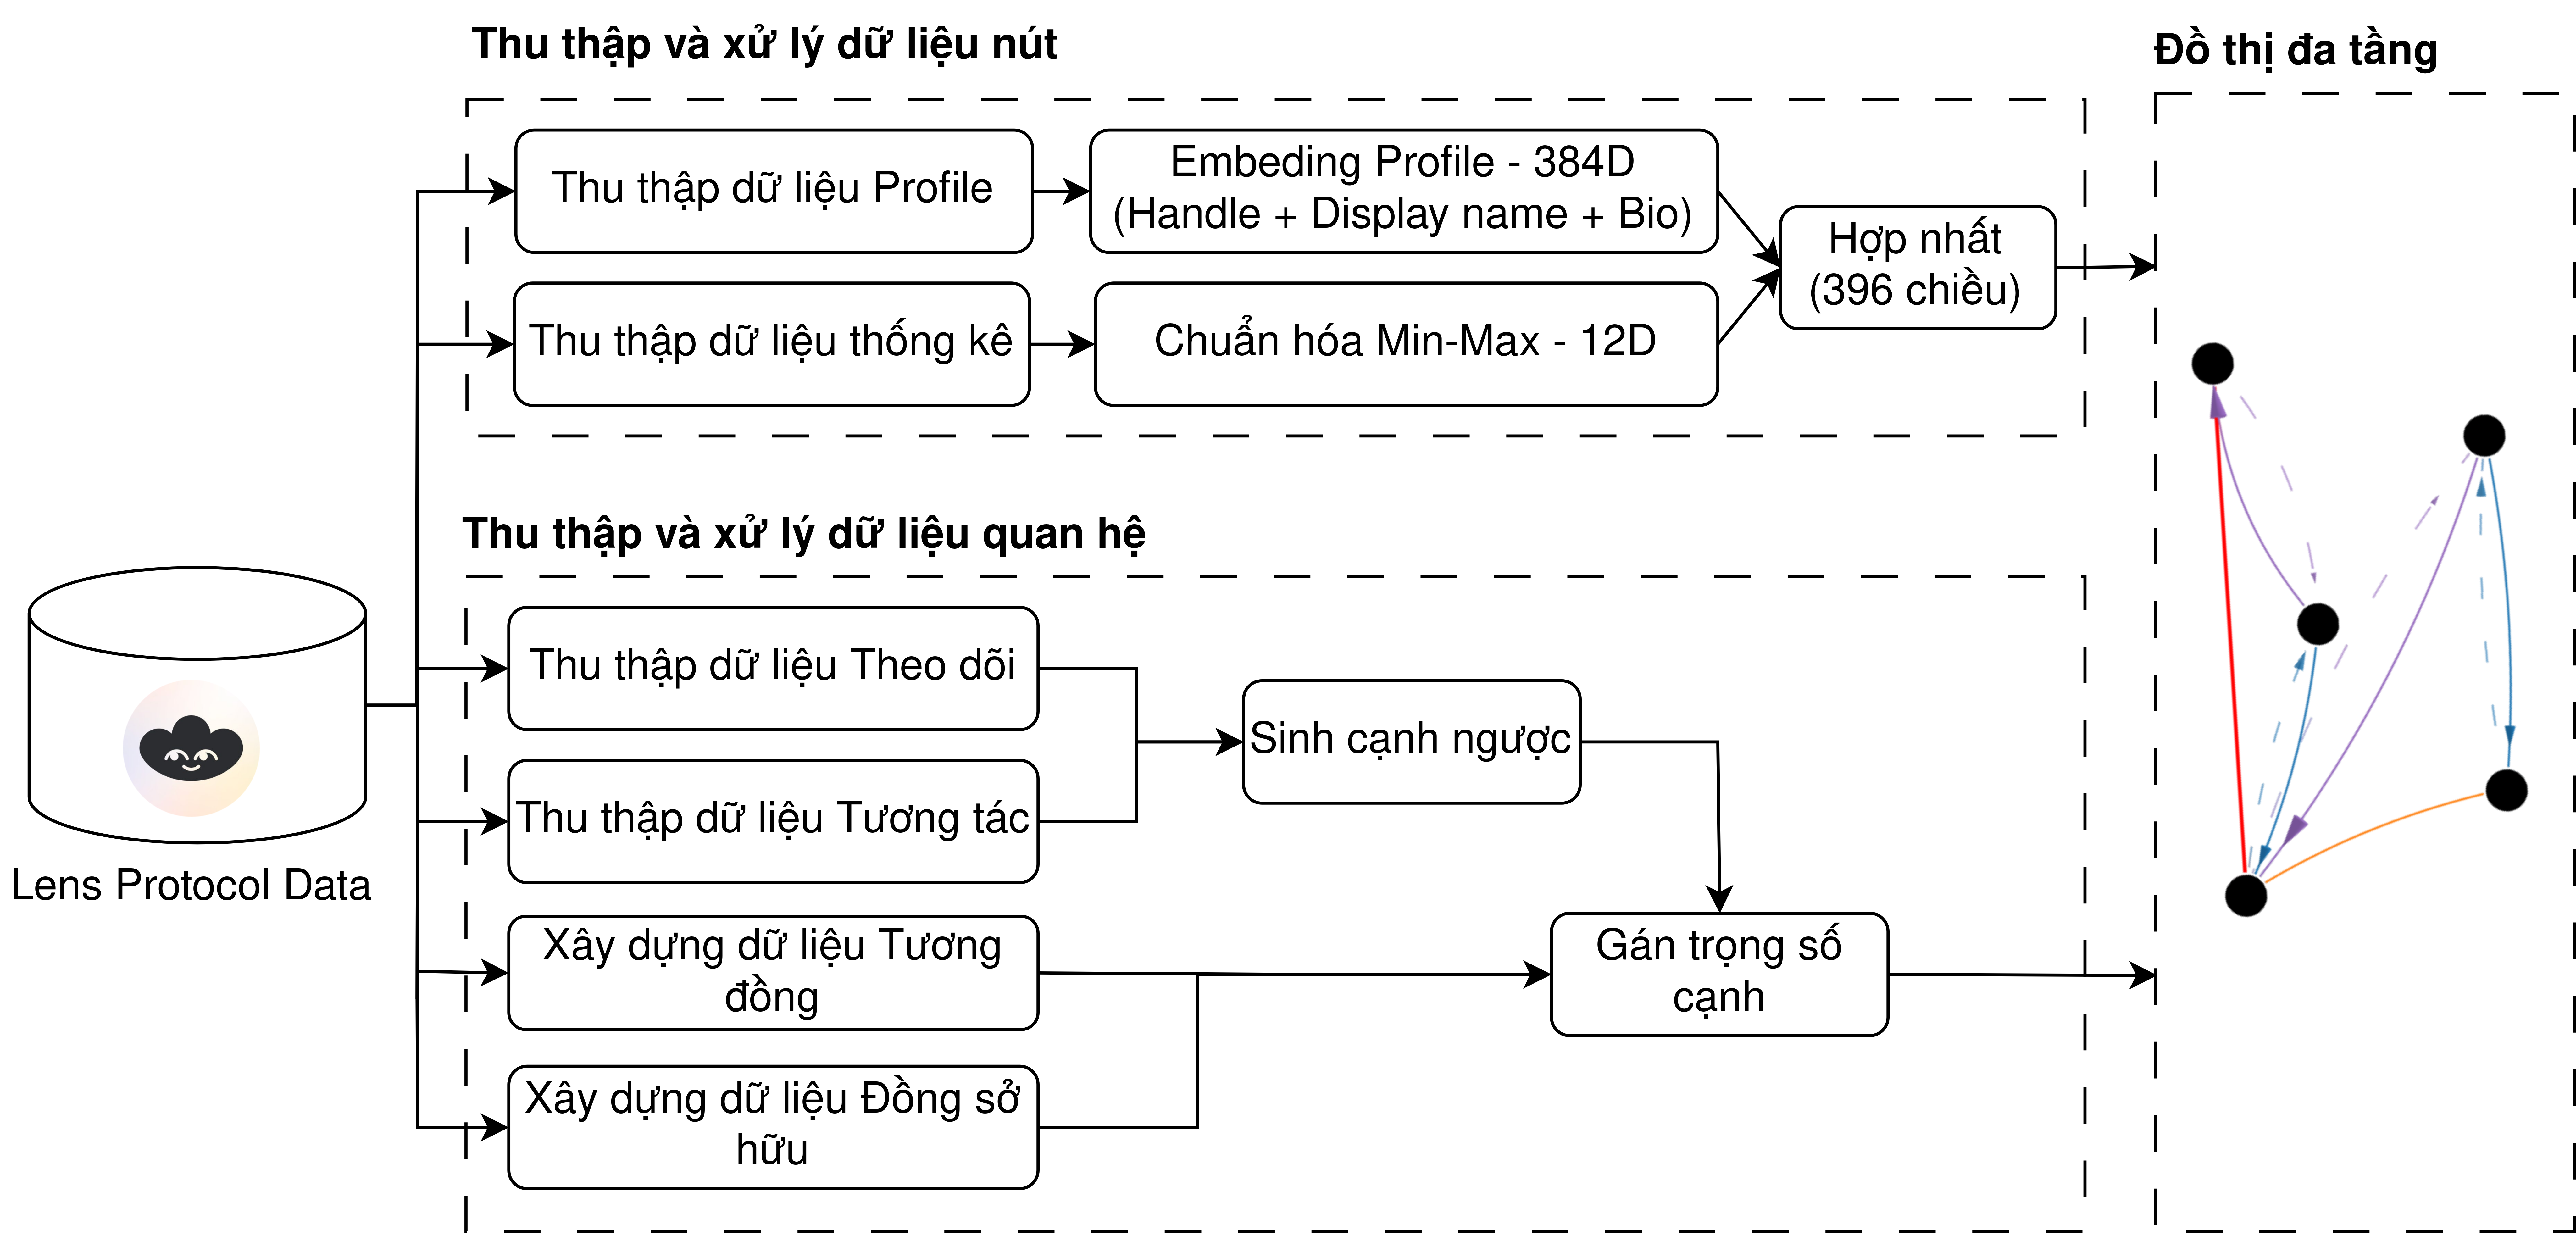
\includegraphics[width=\linewidth]{images/part-02/chap-02/sec-01/BuildMLG.png}
    \vspace{0.3cm}
    \caption{Sơ đồ luồng quy trình thu thập và xây dựng dữ liệu đồ thị đa tầng}
    \label{fig:GraphBuilder}
\end{figure}

\textbf{Đầu vào:} Dữ liệu thô từ mạng lưới Lens Protocol được truy xuất hàng loạt thông qua BigQuery trong một khoảng thời gian xác định, bao gồm thông tin hồ sơ, thống kê hoạt động và các bản ghi sự kiện tương tác.\vspace{0.3cm}

\textbf{Đầu ra:} Một đồ thị đa quan hệ hoàn chỉnh, được đóng gói dưới dạng đối tượng \texttt{Data} của thư viện PyTorch Geometric, sẵn sàng làm đầu vào cho các mạng GNN.\vspace{0.3cm}

\textbf{Quy trình xử lý:}\vspace{-0.1cm}
\begin{itemize}[label={--}, itemsep=3pt]
    \item \textbf{Thu thập và xử lý dữ liệu nút:} Dữ liệu mô tả tài khoản được chia làm hai nhánh trích xuất đặc trưng độc lập trước khi tiến hành hợp nhất:
    \begin{itemize}[label={+}, itemsep=3pt]
        \item \textit{Đặc trưng ngữ nghĩa (Văn bản):} Trích xuất thông tin từ hồ sơ bao gồm Handle, Display Name và Bio. Các trường văn bản này được nhúng qua mô hình \texttt{all-MiniLM-L6-v2} để tạo vector embedding có kích thước 384 chiều.
        \item \textit{Đặc trưng định lượng (12 chiều):} Hệ thống trích xuất 12 biến số liên tục phản ánh độ uy tín và mức độ hoạt động của tài khoản, bao gồm hai nhóm chính:
        \begin{itemize}[label={$\circ$}, itemsep=1pt]
            \item \textbf{11 chỉ số định lượng:} Gồm điểm tin cậy (\texttt{trust\_score}) và 10 chỉ số đo lường quy mô tương tác (tổng số lượt \textit{tips, posts, quotes, reacted, reactions, reposts, collects, comments, followers} và \textit{following}).
            \item \textbf{1 chỉ số thời gian:} Số ngày hoạt động (\texttt{days\_active}), được tính toán dựa trên độ lệch giữa thời điểm tạo tài khoản và thời gian hệ thống hiện tại.
        \end{itemize}
        \indent Để tránh hiện tượng các giá trị có biên độ quá lớn áp đảo quá trình học của mạng nơ-ron, toàn bộ 12 đặc trưng này được đưa qua bộ chuẩn hóa \textit{StandardScaler} để đưa về cùng một phân phối chuẩn (với giá trị trung bình bằng $0$ và độ lệch chuẩn bằng $1$), tạo thành vector định lượng 12 chiều hoàn chỉnh.
        \item \textit{Hợp nhất:} Hai vector trên được ghép nối lại với nhau, tạo thành một vector đặc trưng nút toàn diện với kích thước 396 chiều ($384 + 12 = 396$).
    \end{itemize}

    \item \textbf{Thu thập và xử lý dữ liệu quan hệ:} Dữ liệu liên kết giữa các tài khoản được trích xuất và biến đổi qua ba bước tuần tự để hình thành cấu trúc đa tầng của đồ thị:
    \begin{itemize}[label={+}, itemsep=1pt]
        \item \textit{Thu thập và kiến tạo các tầng quan hệ:} Hệ thống xử lý cơ sở dữ liệu gốc để thiết lập 4 nhóm liên kết. Cụ thể: quan hệ \textbf{Theo dõi} và \textbf{Tương tác} được ánh xạ trực tiếp từ dữ liệu sự kiện trên nền tảng; quan hệ \textbf{Tương đồng} được kiến tạo thông qua thuật toán so khớp chéo tuân thủ nguyên tắc \textit{ràng buộc 2/3} (yêu cầu hai nút phải thỏa mãn 2 trong 3 tiêu chí: tương đồng ngữ nghĩa tiểu sử, khoảng cách Levenshtein của tên định danh, và thời gian tạo); cuối cùng, quan hệ \textbf{Đồng sở hữu} được trích xuất bằng cách kết nối các tài khoản có cùng giá trị tại trường \texttt{owned\_by} (địa chỉ ví sở hữu).
        
        \item \textit{Sinh cạnh ngược (Reverse Edges):} Đối với các tầng quan hệ có hướng (cụ thể là tầng Theo dõi và Tương tác), hệ thống tiến hành sinh thêm các chiều cạnh ngược tương ứng (ví dụ: \texttt{FOLLOW\_REV}). Cơ chế này đảm bảo thông điệp có thể lan truyền linh hoạt theo cả hai chiều trong quá trình huấn luyện GNN. Riêng dữ liệu liên kết của tầng Tương đồng và Đồng sở hữu vốn mang tính chất đối xứng nên được truyền thẳng qua bước tiếp theo.
        
        \item \textit{Gán trọng số cạnh (Edge Weighting):} Sau khi các luồng cạnh gốc và cạnh ngược được hợp nhất, hệ thống tiến hành gán trọng số cơ sở ($W_{base}$) tương ứng cho từng tầng. Cuối cùng, thuật toán áp dụng hàm chuẩn hóa Logarit trên tần suất xuất hiện của hành vi nhằm tinh chỉnh trọng số cuối cùng. Quá trình này giúp đồ thị vừa bảo toàn được sức mạnh của các liên kết mạnh (như quan hệ đồng sở hữu), vừa hạn chế được nhiễu từ các tài khoản siêu đặc.
    \end{itemize}
    
    \item \textbf{Đóng gói thành Đồ thị đa tầng:} Các định danh tài khoản được ánh xạ tuần tự, sau đó các ma trận được đóng gói thành đối tượng đồ thị chuẩn. Đặc biệt, để phân biệt các tầng liên kết khác nhau trong quá trình huấn luyện đa quan hệ, hệ thống truyền vào một vector chỉ mục loại cạnh. Đồ thị hoàn chỉnh bao gồm: ma trận đặc trưng nút \texttt{x}, ma trận liên kết \texttt{edge\_index}, vector trọng số \texttt{edge\_attr} và phân loại cạnh \texttt{edge\_type}.
\end{itemize}
\subsubsection{1.2. Kiến trúc mạng tự mã hóa đồ thị (GAE + GATv2)}

\indent\indent Để giải quyết thách thức về sự thiếu hụt dữ liệu gán nhãn trong giai đoạn đầu, hệ thống áp dụng kiến trúc GAE. Mục tiêu của mô hình này là học không giám sát, tự động nén các đặc trưng đồ thị phức tạp vào không gian nhúng để phục vụ cho thuật toán gom cụm ở bước tiếp theo.\vspace{0.3cm}

Kiến trúc chi tiết của mô hình GAE được minh họa tại \textbf{Hình \ref{fig:GAEPipeline}}. Mô hình được thiết kế với hai thành phần cốt lõi: Bộ mã hóa sử dụng GATv2 và Bộ giải mã.

\begin{figure}[H]
    \centering
    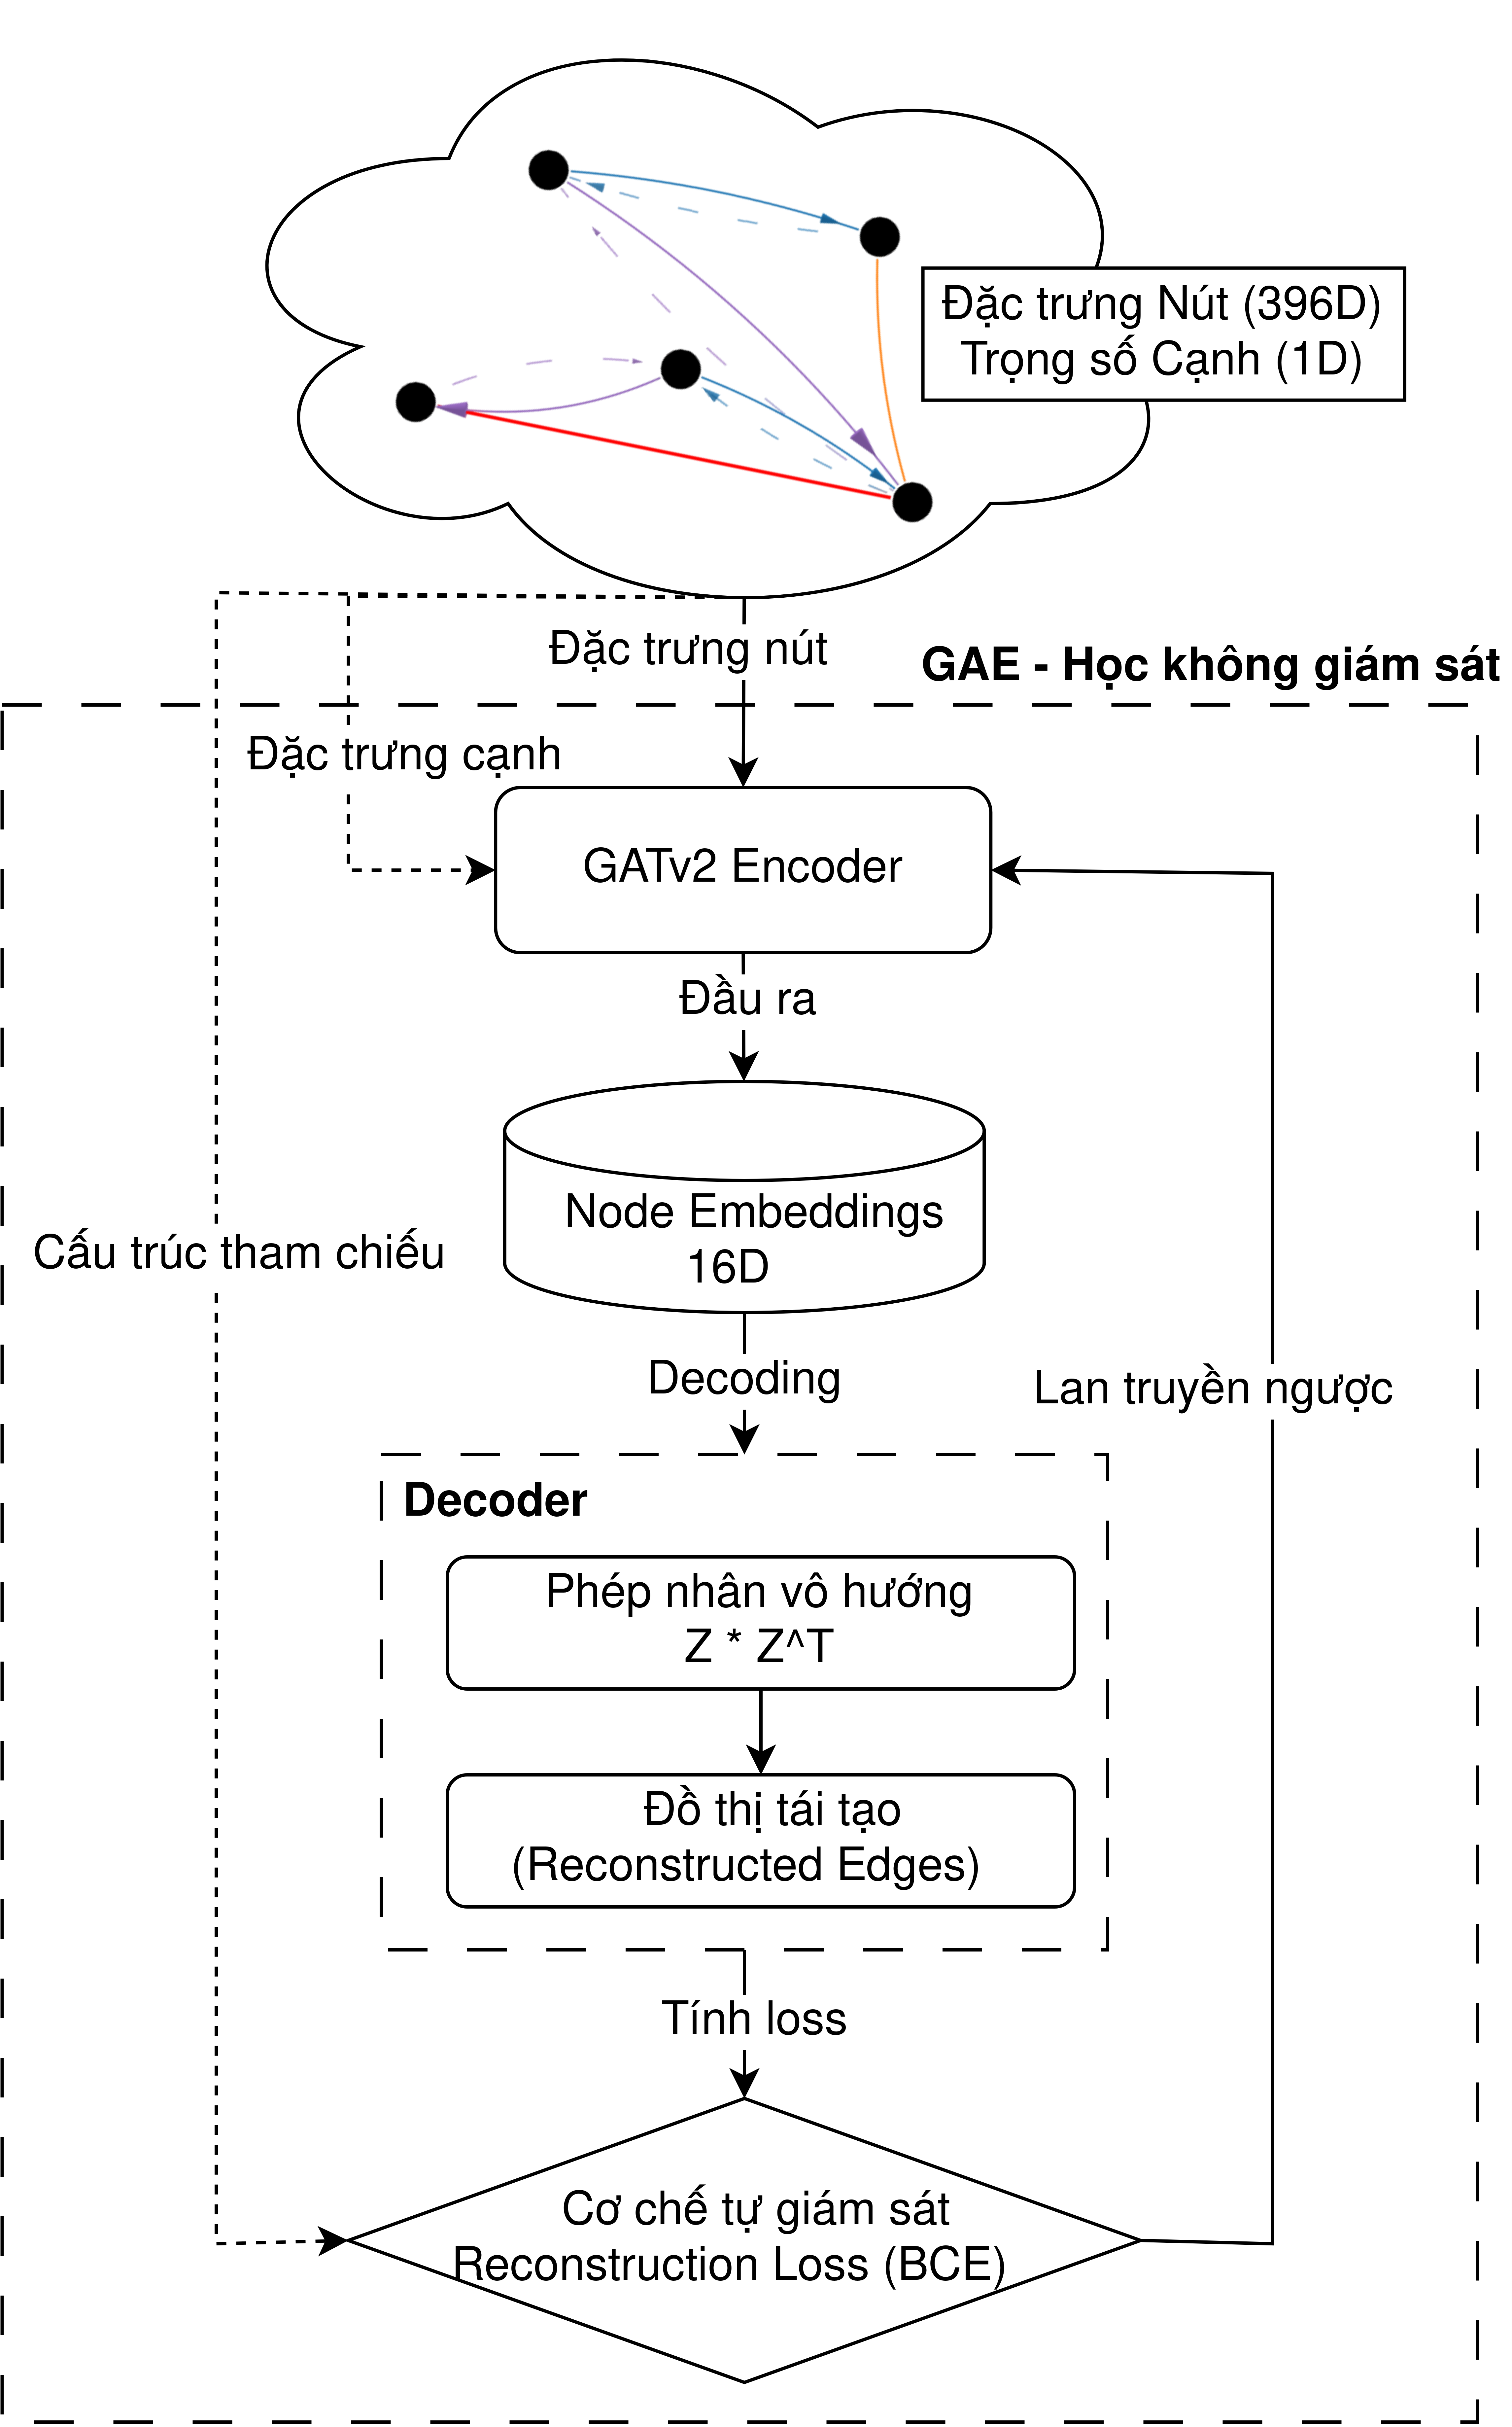
\includegraphics[width=0.6\linewidth]{images/part-02/chap-02/sec-01/GAEPipeline.png}
    \vspace{0.2cm}
    \caption{Kiến trúc Mạng tự mã hóa đồ thị với bộ mã hóa GATv2}
    \label{fig:GAEPipeline}
\end{figure}

\vspace{0.1cm}
\textit{1.2.1. Bộ mã hóa GATv2 Encoder}\vspace{0.2cm}

Hệ thống sử dụng Mạng nơ-ron tích chập đồ thị có cơ chế chú ý phiên bản 2 (\textit{GATv2Conv}) làm bộ mã hóa. Khác với GAT truyền thống, GATv2 sử dụng cơ chế chú ý động (Dynamic Attention), cho phép mô hình xếp hạng độ quan trọng của các nút lân cận một cách linh hoạt hơn. Đặc biệt, bộ mã hóa được thiết kế để duy trì cơ chế Điều hướng chú ý (Attention Steering) thông qua tham số \texttt{edge\_dim=1}, giúp hấp thụ trực tiếp các trọng số cạnh đã được chuẩn hóa Logarit ở giai đoạn trước vào mọi bước nhảy lan truyền.\vspace{0.3cm}

Chi tiết luồng xử lý Tensor qua các tầng của bộ mã hóa được minh họa tại \textbf{Hình \ref{fig:GATEncoder}}:
\begin{figure}[H]
    \centering
    % Đổi tên file ảnh dưới đây cho khớp với sơ đồ GAT Encoder bạn vừa vẽ
    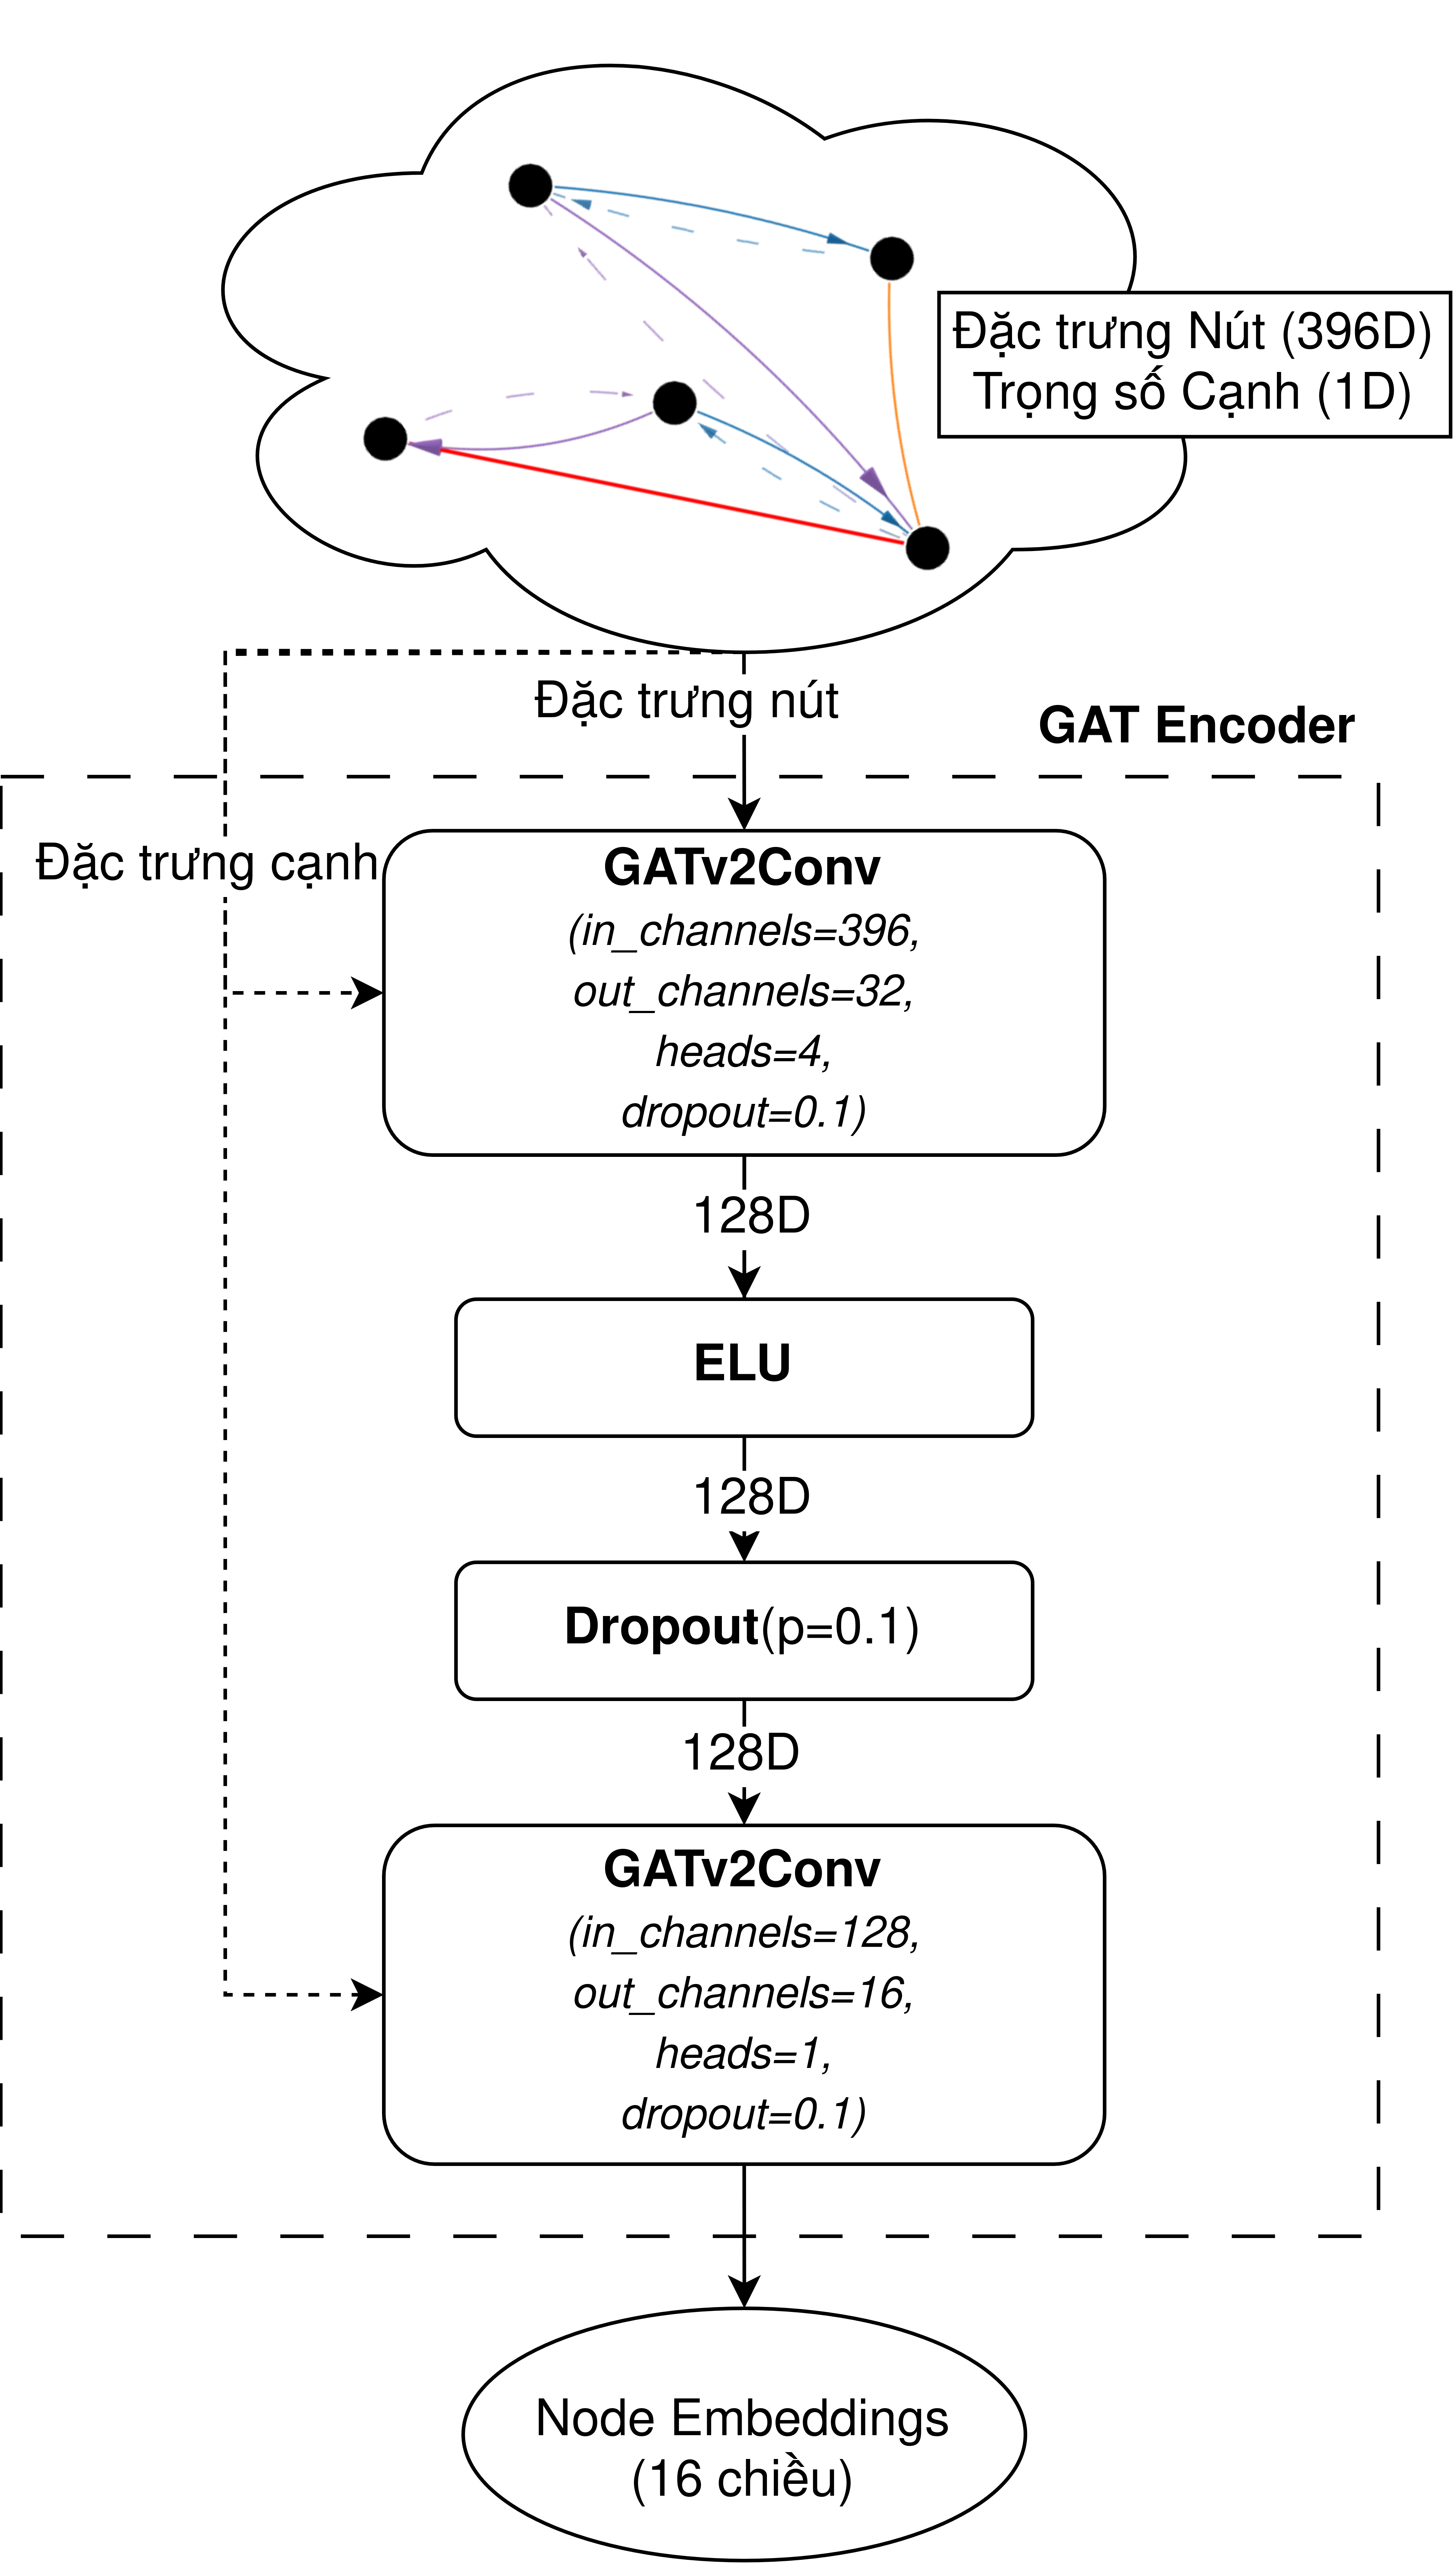
\includegraphics[width=0.6\linewidth]{images/part-02/chap-02/sec-01/GATEncoder.png}
    \vspace{0.2cm}
    \caption{Kiến trúc luồng dữ liệu bên trong Bộ mã hóa GATv2}
    \label{fig:GATEncoder}
\end{figure}

Kiến trúc mã hóa bao gồm hai tầng tích chập:
\begin{itemize}[label={--}, itemsep=3pt]
    \item \textbf{Tầng tích chập thứ nhất (Conv1):} Nhận đầu vào là ma trận đặc trưng $X \in \mathbb{R}^{N \times 396}$. Tầng này sử dụng cơ chế đa chú ý (Multi-head Attention) với $4$ heads nhằm khai phá đặc trưng dưới nhiều không gian biểu diễn khác nhau. Mỗi head ánh xạ dữ liệu thành không gian $32$ chiều. Các kết quả sau đó được ghép nối lại, tạo ra vector trung gian có kích thước $128$ chiều ($32 \times 4$). Đầu ra đi qua hàm kích hoạt phi tuyến ELU (Exponential Linear Unit) và một lớp Dropout với tỷ lệ $0.1$ nhằm ngăn chặn over-fitting.
    \item \textbf{Tầng tích chập thứ hai (Conv2):} Nhận vector $128$ chiều làm đầu vào và thiết lập cơ chế chú ý đơn ($1$ head). Cấu hình này ép buộc mô hình tổng hợp các góc nhìn từ tầng trước để nén thông tin thành vector tiềm ẩn cuối cùng $Z \in \mathbb{R}^{N \times 16}$.
\end{itemize}\vspace{0.3cm}

\textit{1.2.2. Bộ giải mã (Inner Product Decoder)}\vspace{0.2cm}

Thay vì sử dụng một mạng nơ-ron phức tạp, bộ giải mã của GAE tính toán tích vô hướng giữa các vector embedding của các cặp nút ($Z_i \cdot Z_j$) để dự đoán xác suất tồn tại của một cạnh nối giữa chúng. Đầu ra của hệ thống được đánh giá thông qua hàm lỗi tái tạo (\textit{Reconstruction Loss}) dựa trên Binary Cross-Entropy (BCE). Khung học không giám sát này sẽ liên tục sử dụng sai số tái tạo để lan truyền ngược, ép các trọng số của GATv2 phải điều chỉnh sao cho đồ thị tái tạo từ không gian tiềm ẩn gần giống nhất với đồ thị đa quan hệ gốc ban đầu.\vspace{0.3cm}

\textbf{Đầu ra cuối cùng:} Sau khi kết thúc quá trình tối ưu hóa, mô hình trích xuất ma trận có kích thước $N \times 16$ (node embeddings). Ma trận này chứa đựng toàn bộ tri thức về cấu trúc mạng lưới của đồ thị, đóng vai trò là đầu vào tiên quyết cho quy trình phân cụm và gán nhãn giả lập phía sau.